\documentclass[12pt]{report}
\usepackage[a4paper]{geometry}
\usepackage[myheadings]{fullpage}
\usepackage{fancyhdr}
\usepackage{lastpage}
\usepackage{graphicx, wrapfig, subcaption, setspace, booktabs}
\usepackage[T1]{fontenc}
\usepackage[font=small, labelfont=bf]{caption}
\usepackage{fourier}
\usepackage[protrusion=true, expansion=true]{microtype}
\usepackage[ngerman]{babel}
\usepackage{sectsty}
\usepackage{url, lipsum}
\usepackage[utf8]{inputenc}
\usepackage{amsmath}
\usepackage{listings}
\usepackage{float}
\usepackage{hyperref}
\usepackage{multirow}
\usepackage{hyperref}
\usepackage{graphicx}
\usepackage{acronym}

% argmin command for math env
\DeclareMathOperator*{\argmin}{arg\,min}


\newcommand{\HRule}[1]{\rule{\linewidth}{#1}}
\onehalfspacing
\setcounter{tocdepth}{5}
\setcounter{secnumdepth}{5}

%-------------------------------------------------------------------------------
% HEADER & FOOTER
%-------------------------------------------------------------------------------
\pagestyle{fancy}
\fancyhf{}
\setlength\headheight{15pt}
\fancyhead[L]{Robin Baumann, Tom Ganz, Carlo Götz}
\fancyhead[R]{DHBW Karlsruhe}
\fancyfoot[C]{\thepage}
%-------------------------------------------------------------------------------
% TITLE PAGE
%-------------------------------------------------------------------------------

\begin{document}

\title{ \normalsize \textsc{InformatiCup 2018}
		\\ [2.0cm]
		\HRule{0.5pt} \\
		\LARGE \textbf{\uppercase{Intellitank}}
		\HRule{2pt} \\ [0.5cm]
		\normalsize \today \vspace*{5\baselineskip}}

\date{}

\author{
		Robin Baumann, Tom Ganz, Carlo Götz \\
        robin-baumann@outlook.com, \\
        tomganzka@gmail.com, \\
        carlo.goetz@gmail.com \\
		Duale Hochschule Baden-Württemberg, Karlsruhe}

\maketitle
\clearpage
\pagenumbering{roman} 
\tableofcontents
\newpage
\section*{Abkürzungen}
\begin{acronym}
\acro{API}{Application Programming Interface}
\acro{ARMA}{Autoregressive-Moving Average}
\acro{CLI}{Command Line Interface}
\acro{CORS}{Cross-Origin Resource Sharing}
\acro{CSV}{Comma Separated Values}
\acro{DI}{Dependency Injection}
\acro{HTTP}{Hypertext Transfer Protocol}
\acro{IOC}{Inversion Of Control}
\acro{JSF}{Java Server Faces}
\acro{JSON}{Javascript Object Notation}
\acro{MAE}{Mean Absolute Error}
\acro{OSM}{Open Street Map}
\acro{RDBMS}{Relational Database Management System}
\acro{RMSE}{Root Mean Squared Error}
\acro{SPA}{Single Page Application}
\end{acronym}
\newpage
%-------------------------------------------------------------------------------
% Section title formatting
\sectionfont{\scshape}
%-------------------------------------------------------------------------------

%-------------------------------------------------------------------------------
% BODY
%-------------------------------------------------------------------------------
\pagenumbering{arabic}
\setcounter{page}{1}
\section*{Motivation und Zusammenfassung}
Das Auto ist in Deutschland das Fortbewegungsmittel Nummer 1. Einer Umfrage des Umweltbundesamtes (UBA) zufolge sind 37 Prozent der Menschen in Deutschland (ab 14 Jahre) täglich mit dem Kfz unterwegs \cite{fortbewegung}. Auch wenn die Elektromobilität stark auf dem Vormarsch ist, besitzen die meisten Deutschen noch ein Fahrzeug mit einem Verbrennungsmotor. Durch die in dieser Arbeit beschriebene Lösung zum 13. InformatiCup der Gesellschaft für Informatik e.V. wird es ermöglicht, die benötigten Tankstopps Benzinpreis-optimal zu planen, um so bares Geld zu sparen. Es wird eine vorausschauende und intelligente Tankstrategie für eine gegebene Route berechnet, welche den Gesamtpreis für Kraftstoffe minimiert. Das entwickelte System ist für den Alltagsverkehr geeignet, da es aufgrund von Zeit- und Ortsangaben, wie sie beispielsweise in einem Kalender gehalten werden, die optimale Tankstrategie berechnet. Dies geschieht durch ein Maschinenlernmodell, welches auf historischen Benzinpreisen von 15.000 Tankstellen in Deutschland der letzten fünf Jahre trainiert wird. Das Entwickelte System kann Benzinpreise vorhersagen und so für Wochen im Voraus die optimale Tankstrategie finden. 


\chapter{Theoretische Grundlagen}
\section{Fixed-Path-Gas-Station Problem}

Die hier verwendete Tankstrategie wurde implementiert nach dem Algorithmus aus der Publikation 'To Fill or Not To Fill'\cite{fixedgas}.
Gegeben sei eine Route, welche definiert ist durch eine Menge von Tankstellen und eine maximale Tankkapazität des Fahrzeuges.
Jede Tankstelle ist abzufahren, wobei die erste Tankstelle dem Startpunkt der Route entspricht.
Dadurch ergibt sich folgender Algorithmus:
\begin{enumerate}
\item Sei $b$ die aktuelle Position gegeben durch eine Tankstelle
\item Sei $l$ eine Liste von Tankstellen die durch die maximale Tankkapazität von $b$ aus erreichbar sind
\item Sortiere die Liste nach den Benzinpreisen und der Nähe zum Ziel aufsteigend
\item Tanke genau so viel, dass die günstigste (erste) Tankstelle $c$ aus $l$ erreicht wird
\item Falls $c$ nicht die End-Tankstelle ist, wiederhole Punkt $1$
\end{enumerate}

Ebenfalls benutzen wir eine naive Tankstrategie (immer volltanken) um sie mit unserer zu vergleichen. Der Algorithmus wird beschrieben durch:

\begin{enumerate}
\item Sei $l_{i=0}$ die aktuelle Position gegeben durch eine Tankstelle
\item Tanke voll (Kapazität-Füllstand)
\item Erreiche die nächste Tankstelle $l_{i+1}$
\item Tanke die während der Distanz von $l_{i}$ nach $l_{i+1}$ verbrauchten Liter wieder auf
\item Falls $l_{i+1}$ nicht die End-Tankstelle ist, wiederhole Punkt $3$
\end{enumerate}

Die Distanz zwischen zwei Tankstellen wird mittels der Haversine-Formel zwischen zwei Geo-Punkten berechnet \cite{haversine}.

\section{Zeitreihenanalyse}
\section{Regression in Machine Learning}


\chapter{Implementierungsdetails}
Zur Lösung der Aufgabenstellung wurde eine Software entwickelt, deren Aufbau im Folgenden beschrieben wird. Das Design und die Implementierung der Anwendung kann in die Teile Backend, Frontend, Fixed-Path-Gas-Station-Problem und Preisvorhersage unterteilt werden. Die einzelnen Teile werden in den nächsten Abschnitten jeweils erläutert.

\section{Backend}
Das Backend hat die Aufgabe, die benötigten Daten für das Frontend bereitzustellen. Zur Kommunikation zwischen Front- und Backend wird  \ac{HTTP} in Verbindung mit dem Datenformat \ac{JSON} verwendet. Das Backend ist dabei nicht für die Generierung einzelner Teile des Frontends zuständig, wie es bei Technologien wie \ac{JSF} der Fall ist.

Diese Entkoppelung ermöglicht die Implementierung weiterer spezialisierter Frontends. So wäre zum Beispiel die Entwicklung eines Frontends für Mobilgeräte ohne große Anpassungen des Backends möglich.

Für die Umsetzung des Backends wurde die Programmiersprache Java gewählt. Java bietet viele Open Source Bibliotheken, die die Entwicklung der Problemlösung unterstützen und beschleunigen können. Neben der großen Auswahl an Bibliotheken, bietet Java sowohl ausreichende Performance als auch viele Werkzeuge, die den Entwicklungsprozess vereinfachen. Durch die Plattformunabhängigkeit ist es auch möglich, dass die Entwicklung auf jedem der im Team eingesetzten Betriebssysteme reibungslos und ohne spezielle Anpassungen möglich ist.

Im nächsten Abschnitt wird auf die Architektur des Backends eingegangen.

\subsection{Architektur}

\begin{figure}
\centering
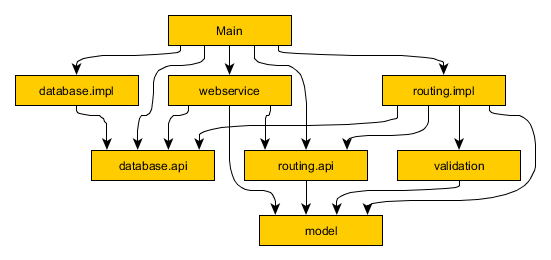
\includegraphics[width=1\linewidth]{architecture.png}
\caption{Abhängigkeiten der einzelnen Packages des Backends}
\label{fig:arch}
\end{figure}

Abbildung \ref{fig:arch} zeigt die Architektur des Backends. Es werden die einzelnen Packages und ihre Abhängigkeiten untereinander aufgeführt. \texttt{Main} ist die einzige Klasse, die nicht in einem weiteren Sub-Package enthalten ist und wird deshalb separat aufgeführt.

Zur Aufgabe von \texttt{Main} gehört es, die Applikation zu starten und die Implementierungen der einzelnen Interfaces zu instanziieren. Durch Verwendung des \ac{IOC}-Prinzips wird sichergestellt, dass die einzelnen Sub-Packages jeweils nur vom Interface abhängen und nicht von einer konkreten Implementierung des Interfaces. Die Abhängigkeiten einer Klasse werden zur Laufzeit per Constructor-Injection zur Verfügung gestellt. Auf die Verwendung eines \ac{DI}-Containers wurde verzichtet, da er bei dieser Programmgröße und -komplexität keine Vorteile bringt.

Ein Nebeneffekt dieser Aufteilung ist die Möglichkeit, Unit Tests für die einzelnen Klassen zu schreiben ohne zum Beispiel eine aktive Datenbankverbindung zu benötigen. Über Mocking Bibliotheken kann in Tests statt einer konkreten Implementierung eines Interfaces ein Mock Objekt konstruiert und verwendet werden. Das Mock Objekt kann mit dem für den Test nötigen Verhalten konfiguriert werden.

Die folgenden Abschnitte erläutern jeweils die Aufgabe der einzelnen Packages.

\subsubsection{model}
\label{sec:model}

Im Package \texttt{model} werden Klassen definiert, die für den Datenfluss im Programm notwendig sind. Die enthaltenen Klassen definieren die Daten der Problemdomäne (Domain Layer), der externen \ac{HTTP}-\ac{API} (Web Layer) und der Datenbank (Persistence Layer). Auf eine weitere Unterteilung der Klassen und Einteilung in die entsprechenden Layer wurde bewusst verzichtet. Der Vorteil einer Einteilung in die verschiedenen Layer hätte den Vorteil, dass sich die Datendefinitionen der einzelnen Layer unabhängig voneinander entwickeln können. Dies würde allerdings bedeuten, dass zwischen den einzelnen Layern eine Übersetzung stattfinden müsste. Diese Unterteilung könnte bei Bedarf vorgenommen werden.

Die Entscheidung für ein Anemic Domain Model wurde bewusst getroffen und soll eine spätere Einteilung der Klassen in die Layer erleichtern.

\subsubsection{webservice}
\label{sec:webservice}

Das Package \texttt{webservice} enthält die Klassen \texttt{Router} und \texttt{ApiHandler}. \texttt{Router} ist für die Konfiguration der Bibliothek Spark zuständig. Spark ist ein Micro Framework zur Erstellung von Web Anwendungen. Da Spark alle Anforderungen der Anwendung in diesem Bereich erfüllen kann, wurde auf den Einsatz von Spring oder der JavaEE-Spezifikation in Verbindung mit einem Application Server verzichtet, um die Komplexität dieser Varianten zu vermeiden.

In \texttt{Router} werden unter anderem die Routen der \ac{HTTP}-\ac{API} mit den entsprechenden Methoden der Klasse \texttt{ApiHandler} verknüft. Des Weiteren wird für die lokale Entwicklung \ac{CORS} aktiviert. Dies ermöglicht die Bereitstellung des Frontends während der Entwicklung von einem anderen Host (Webpack Dev Server) aus. Dadurch ist es nicht nötig, bei Änderungen des Frontends den Java-Build zu verwenden und verringert so die Feedback Loop.

Die Klasse \texttt{ApiHandler} ist für die Deserialisierung der Daten aus der Web Request zuständig. Die deserialisierten Daten werden anschließend an die Services des Domain Layers übergeben. Das Ergebnis dieser Operation wird schließlich wieder serialisiert. Sollten während der Bearbeitung der Anfragen Exceptions auftreten, werden diese an dieser Stelle auch in Instanzen der Klasse \texttt{ProblemResponse} umgewandelt. \texttt{ProblemResponse} richtet sich nach \cite{nottingham} und bietet so ein konsistentes Vorgehen zur Übermittlung von Fehlern des Backends.

\subsubsection{routing}
\label{sec:routing}

Das Package \texttt{routing}, mit seinen Sub Packages \texttt{api} und \texttt{impl}, ist für die Lösung der eigentlichen Aufgabe der Anwendung zuständig. Konkret bedeutet das, dass sowohl die Tankstrategien als auch die Preisvorhersagen hier berechnet werden. Durch die Trennung in \texttt{api} und \texttt{impl} ist es möglich, dass der Web Layer nicht von einer konkreten Implementierung der Logik abhängig ist. Bei der Implementierung dieses Layers wurde die Konvention verwendet, dass Fehler in den Eingabedaten durch Java's Checked Exceptions Mechanismus ein Bestandteil der \ac{API} werden. Dies macht den Kontrollfluss explizit.

Der \texttt{SimpleRoutingService} verwendet das Strategy Pattern \cite{gof}, um den verwendeten Algorithmus bei Bedarf durch einen anderen zu ersetzen.

Die Preisvorhersage verwendet ein Model der Bibliothek H2O. Dieses Model wird aus den \texttt{resources} geladen und beinhaltet das Ergebnis des Trainings. Mit dem Model wird ein Predictor instanziiert, der wiederum den Preis gemäß der Anfrage vorhersagt.

\subsubsection{database}
\label{sec:database}

Das Package \texttt{database} definiert die Schnittstelle zur Datenbank und bietet eine konkrete Implementierung für eine Postgresql Datenbank an. Hierzu werden die Bibliotheken HikariCP und sql2o verwendet. Die Aufgabe von HikariCP ist es, einen Connection Pool für die Datenbank Verbindungen zur Verfügung zu stellen. Die Bibliothek sql2o bietet hingegen die Möglichkeit, das Ergebnis einer Datenbankabfrage in Instanzen der entsprechenden Klassen zu deserialisieren. Eine Besonderheit von sql2o ist die Verwendung von SQL Statements, die im jeweiligen Dialekt der Datenbank verfasst werden. Im Gegensatz zu Bibliotheken wie Hibernate bedeutet dies, dass zur Unterstützung einer neuen Datenbank sämtliche Queries angepasst werden müssen. Allerdings ermöglicht die Verwendung des Datenbank-spezifischen Dialekts auch eine Nutzung der Datenbank-spezifischen Features.

\subsection{Persistenz}

Als \ac{RDBMS} wird Postgresql eingesetzt. Postgresql ist nicht nur Open Source, sondern verfügt auch über eine Erweiterung für Geodaten: PostGIS. Dadurch war es möglich, die vorhandenen Daten über Tankstellen mit weiteren Daten zu erweitern, um möglichst viele Features für die Preisvorhersage zu erhalten.

Das genaue Vorgehen zur Ermittlung der Daten wurde in der Datei \texttt{orga.org} genau dokumentiert. Damit diese recht zeitintensiven Schritte nicht wiederholt werden müssen, liegt diesem Dokument eine Sicherung der kompletten Datenbank bei.

Im laufenden Betrieb sind nur wenige Tabellen der Datenbank notwendig. Die Tabelle \texttt{stations} ist die wichtigste Tabelle, denn sie enthält die Daten zu den einzelnen Tankstellen. Tabelle \ref{tab:stations} zeigt die verwendeten Spalten.

\begin{table}[h]
	\centering
	\begin{tabular}{l l l}
		\textbf{Spalte} & \textbf{Type} & \textbf{Bemerkungen} \\ 
		\hline \hline
		id & smallint & Id wie in Eingabedaten \\
        lat & double & Breitengrad in WGS84 \\
        lon & double & Längengrad in WGS84 \\
        station\_name & varchar(255) & Name \\
        street & varchar(255) & Adresse \\
        house\_number & varchar(255) & Hausnummer \\
        zip\_code & varchar(5) & PLZ  \\
        city & varchar(255) & Ort \\
        brand & varchar(255) & Marke  \\
        brand\_no & int & Id der Marke \\
        bland\_no & int & Id des Bundeslands \\
        kreis & varchar(12) & Verwaltungsschlüssel des Landkreises \\
        abahn\_id & int & Id der nächsten Autobahn \\
        bstr\_id & int & Id der nächsten Bundesstraße \\
        sstr\_id & int & Id der nächsten Schnellstraße \\
		\hline 
	\end{tabular}
	\caption{Im Backend verwendete Spalten der Tabelle stations}
	\label{tab:stations}	
\end{table} 

Neben den Informationen, die bereits in den Daten von Tankerkönig enthalten waren, wurden die Tankstellen mit weiteren Daten versehen. Ein großer Teil der zusätzlichen Daten wurde aus Daten von \ac{OSM} gewonnen. Auf diese Daten wird im nächsten Abschnitt genauer eingegangen.

\subsubsection{Geodaten}

Um weitere Features der Tankstellen zu gewinnen, wurden die \ac{OSM} Daten von Deutschland verwendet. Hierzu wurden Daten zu Autobahnen, Bundes- und Schnellstraßen und den Verwaltungsgrenzen aus dem \ac{OSM} Datensatz extrahiert.

Die Informationen zu nahegelegenen Autobahnen, Bundes- und Schnellstraßen wurden mithilfe der Hilfstabellen \texttt{bundesstr}, \texttt{autobahn} und \texttt{schnellstr} ermittelt. Zuerst wurden die entsprechenden Daten aus dem \ac{OSM} Datensatz in diese Tabellen geschrieben. Anschließend wurden die enthaltenen Geometrien von der Projektion \texttt{EPSG:4326} (\texttt{WGS84}) in \texttt{EPSG:4839} umgewandelt. Auch die Punktgeometrien der Tankstellen wurden konvertiert. Funktionen, die mit der Distanz zwischen zwei Geometrien arbeiten, verwenden in PostGIS immer die Einheit der Projektion. Die Einheit von \texttt{EPSG:4326} ist Grad und somit für die Berechnung von Distanzen in Metern ungeeignet. \texttt{EPSG:4326} hingegen verwendet Meter und hat eine Genauigkeit von etwa 1 Meter im betrachteten Bereich. Dies ist für die Anforderungen ausreichend. Auf den Geometriespalten wurde jeweils ein Spatial Index erstellt, um die Suche nach nahegelegenen Geometrien zu beschleunigen. Anschließend wurden die Tankstellen mit den Geometrien der verschiedenen Straßen gejoined. Als Bedingung für den Join wurde eine Distanz kleiner 5000 Meter verwendet. Dies bedeutet, dass die entsprechende Spalte in der Tabelle \texttt{stations} den Wert \texttt{null} aufweist, falls sich kein Teil einer Straße in mindestens 5 km Nähe befindet.

Um die Zugehörigkeit zu einem Landkreis und Bundesland festzustellen, wurden die Informationen über Gemeindegrenzen aus den \ac{OSM} Daten extrahiert und in die Hilfstabellen \texttt{bundeslaender} und \texttt{kreise} gespeichert. Die enthaltenen Geometrien wurden mit der Funktion \texttt{ST\_polygonize} in Polygone umgewandelt. Dieser Schritt ist notwendig, um mit der Funktion \texttt{ST\_contains} zu ermitteln, ob eine Tankstelle in einem Bundesland bzw. Kreis liegt. Auch hier wurde die Abfragegeschwindigkeit durch die Verwendung von Spatial Indices erhöht.

\subsection{Tests}

Um während der Entwicklung die Korrektheit des Programms sicherzustellen, wurden Tests implementiert. Es wurden Unit Tests implementiert, um komplexere Klassen zu testen. Unit Tests enden mit dem Suffix \texttt{Test}.

Neben den Unit Tests wurden mehrere Integration Tests implementiert. Diese Integration Tests enden mit dem Suffix \texttt{IT}. Die Integration Tests erfordern eine aktive Datenbank Verbindung und werden deshalb während des Builds nicht ausgeführt. Um die Tests mit Maven zu starten, kann das Maven Profil \texttt{it} aktiviert werden. Dies kann mit dem Kommandozeilenargument \texttt{-P it} erreicht werden.

Um den verwendeten Algorithmus gegen die naive Tankstrategie zu benchmarken kann die Klasse \texttt{FixedVsNaiveIT} verwendet werden. Diese Klasse instanziiert den \texttt{ApiHandler} zwei mal und verwendet jeweils eine unterschiedliche Tankstrategie. Anschließend wird der Gesamtpreis verglichen.

\newpage
\section{Frontend}

Das Frontend stellt die Schnittstelle der Anwendung zum Benutzer dar. Ein Benutzer kann über das Frontend die verschiedenen \ac{CSV} Dateien einlesen. Die Daten werden anschließend zur Bearbeitung an das Backend gesendet. Das Ergebnis wird schließlich im Frontend dargestellt.

\subsection{Design}

Abbildung \ref{fig:startview} zeigt die Ansicht, die der Benutzer beim ersten Aufruf der Anwendung sieht. Der Bereich ist in zwei Teile aufgeteilt. Oben wird der Titel des Programms angezeigt, sowie ein Button \texttt{Menu} angeboten, um das seitliche Menü auszuklappen. In diesem Zustand ist das Menü leer. Der zweite Bereich besteht aus einer Kartenansicht und einem Button \texttt{Actions}. Die Karte soll beim Start auf die aktuelle Position des Benutzers, falls vorhanden, zentriert werden. Ansonsten erfolgt eine Zentrierung auf Karlsruhe. Der Button \texttt{Actions} ist der zentrale Anlaufpunkt für den Benutzer, um die Anwendung zu verwenden. Ein Click auf den Button lässt zwei weitere Buttons erscheinen, um Dateien zur Ermittlung einer optimalen Route bzw. einer Preisvorhersage an die Anwendung zu übermitteln. Dieser Zustand wird in Abbildung \ref{fig:draweropen} gezeigt.

Neben den Buttons zur Übermittlung von Dateien, zeigt diese Abbildung auch das seitliche Menü mit Inhalt. Der Button \texttt{<<} dient dazu das Menü wieder zu schließen. Wenn der Benutzer eine Route anfragt, wird das Ergebnis im Seitenmenü dargestellt. Dazu wird ein Abschnitt Routen erstellt, der sich bei Bedarf einklappen lässt. Dieser Bereich enthält für jede einzelne Anfrage des Benutzers das jeweilige Ergebnis in Tabellenform. Unter der Tabelle wird jeweils ein Button zum Download der Ergebnis-\ac{CSV} und zum Löschen der Route angeboten. Eine Route wird auf der Karte durch Punkte für die angefahrenen Tankstellen angezeigt. Diese Punkte sind miteinander verbunden. Der Abschnitt zur Anzeige von Preisvorhersagen soll dazu analog funktionieren. Allerdings werden die angefragten Tankstellen als einzelne Punkte angezeigt. Am unteren Bildschirmrand ist die Anzeige eines Fehlers zu sehen. Es wird dem Benutzer eine kurze Information gegeben, die er mit einem Click auf den Button \texttt{x} schließen kann.

\begin{figure}
\centering
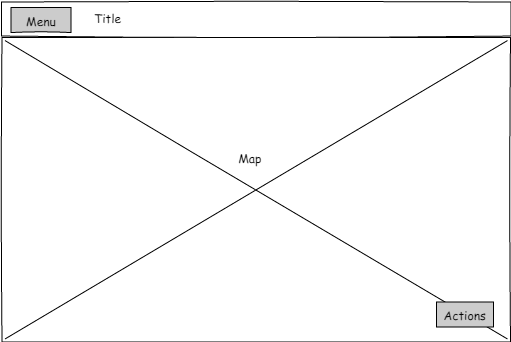
\includegraphics[width=0.7\linewidth]{startview.png}
\caption{Start Ansicht des Frontends}
\label{fig:startview}
\end{figure}

\begin{figure}
\centering
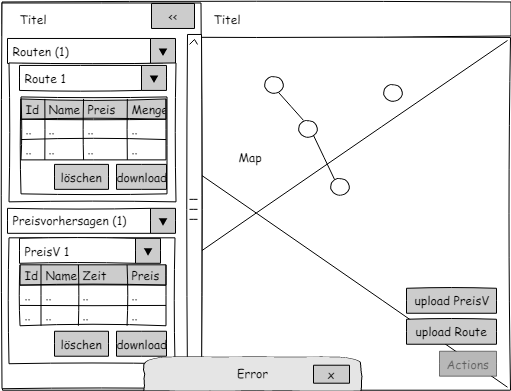
\includegraphics[width=0.7\linewidth]{draweropen.png}
\caption{Frontend während Verwendung}
\label{fig:draweropen}
\end{figure}

\subsection{Implementierung}

Zur Implementierung des Frontends wurde auf Web-Technologien gesetzt. Dies erlaubt eine kurze Feedback Loop bei der Entwicklung. Zur Entwicklung wurde die Sprache TypeScript verwendet. Bei TypeScript handelt es sich um ein Superset von Javascript, das um ein starkes Typsystem erweitert wurde. Durch die starke Typisierung ist es möglich, bereits während der Entwicklung Fehler zu erkennen, die bei der Verwendung von JavaScript erst zur Laufzeit auftreten.

Zu den nennenswerten eingesetzten Bibliotheken zählen OpenLayers 4 zur Darstellung von Karten, vue.js als Framework zur Erstellung von \acp{SPA} und vue-material als Komponenten Bibliothek.

Die Anwendung wurde in vue.js Komponenten unterteilt. Diese Komponenten befinden sich im Ordner \texttt{frontend/vue} und bestehen jeweils aus einer \texttt{.html} und einer \texttt{.ts} Datei. Die \texttt{.ts} Datei definiert das Verhalten der Komponente und die \texttt{.html} Datei das Aussehen.

Die Hauptkomponente, die die untergeordneten Komponenten instanziiert und für die Orchestration der Anwendung zuständig ist, befindet sich in den Dateien \texttt{index.ts} und \texttt{index-template.html}. Funktionalitäten, die nicht die Darstellung der Benutzeroberfläche beeinflussen, wurden im Ordner \texttt{frontend/app} abgelegt.

Die Darstellung der Karte verwenden OpenLayers 4. Die angezeigte Basiskarte ist von \ac{OSM} und erfordert eine aktive Internetverbindung während der Verwendung der Anwendung.

Während der Entwicklung der Anwendung kann der Webpack Dev Server mit dem Script \texttt{start} über das Tool yarn gestartet werden. Der Dev Server erstellt das Frontend nach Änderungen am Quellcode neu und triggert einen Reload des Browsers, falls nötig. Für die Auslieferung der Anwendung startet der Maven Build das Script \texttt{build} und kopiert die resultierenden Dateien in den Ordner \texttt{resources/public}. Spark ist so konfiguriert, dass der Inhalt dieses Ordners als statischer Inhalt zur Verfügung steht.

\subsection{Tests}

Für das Frontend wurden keine automatisierten Tests implementiert. Aufgrund der Überschaubarkeit der Anwendung wurde hierbei auf ein manuelles Testprotokoll zurückgegriffen. Das Testprotokoll beinhaltet folgende Schritte:

\begin{enumerate}
\item Frontend öffnen
\item Action Route Uploaden aufrufen
\item Prüfen, ob Karte auf Route zoomt
\item Prüfen, ob Ergebnis in seitlichem Menü angezeigt wird
\item Action Preisvorhersage Uploaden aufrufen
\item Prüfen, ob Karte auf angefragte Tankstellen zoomt
\item Prüfen, ob Ergebnis in seitlichem Menü angezeigt wird
\item Weitere Route hinzufügen
\item Erste Route löschen
\item Prüfen, ob erste Route nicht mehr in Ergebnisliste ist
\item Weitere Preisvorhersage hinzufügen
\item Erste Preisvorhersage löschen
\item Prüfen, ob erste Route nicht mehr in Ergebnisliste ist
\item Action Route Downloaden aufrufen
\item Prüfen, ob CSV korrekt ist
\item Action Preisvorhersage Downloaden aufrufen
\item Prüfen, ob CSV korrekt ist
\end{enumerate}

\subsection{Einschränkungen}

Während der Entwicklung wurde der aktuellste Chrome Browser von Google verwendet. Andere Browser werden momentan nicht unterstützt. Zum Zeitpunkt der Erstellung dieser Dokumentation, ist zumindest ein Bug in Firefox bekannt, der das Downloaden von Routen verhindert.



\section{Datenverarbeitung / Preisvorhersage}
In diesem Kapitel werden unsere Entscheidungen bezüglich der verwendeten Lernalgorithmen und der Datenverarbeitung dokumentiert. 
\subsection{Feature Engineering}
Der erste Vorbereitungsschritt war, die vorhandenen Daten auf eine einheitliche Frequenz zu bringen. Um dies zu erreichen, wurde eine Datenbanktabelle mit stündlichen Zeitstempeln von Beginn der Aufzeichnung an bemustert. Anschließend wurde für jeden Zeitstempel ein Preis $p(t)$ nach folgendem Kriterium eingetragen:
\begin{equation*}
p(t) = \begin{cases}
p_{neu}, & \text{falls für } [t, t+1] \text{ ein neuer Preis $p_{neu}$ vorhanden ist}\\
p(t-1), & \text{sonst} 
\end{cases}
\end{equation*}

Dieses Grundgerüst eines Feature-Vektors wurde um die in \autoref{tab:features} aufgeführten zusätzlichen Merkmale erweitert. Durch die Persistierung der Daten in einer Datenbank kann effizient darauf zugegriffen werden. Bei den vorhandenen Datenmengen wäre ein Verbund mehrerer Datenbanktabellen zu zeitaufwendig, weshalb die redundante Speicherung mancher Daten in Kauf genommen wird. Für das Training des Regressionsalgorithmus wird aus dem Datensatz eine Trainingsmenge mit 75\% des gesamten Datensatzes erstellt. Die restlichen 25 \% ergeben die Testmenge zur Validierung unseres Modells.

\begin{table}
	\centering
	\begin{tabular}{l r}
		\textbf{Merkmal} & \textbf{Ursprung} \\ 
		\hline \hline
		Feiertage & \texttt{holidays} Python Package  \cite{holidays} \\ 
		Schulferien &  Schulferien.org \cite{ferien} \\ 
		Bundesland & 
        \multirow{3}{*}{ $\Bigg\}$ OpenStreetMap \cite{osm}}\\
        Landkreis &\\
        nächste Hauptverkehrsstraße & \\
		\hline 
	\end{tabular}
	\caption{Auflistung der zusätzlich verwendeten Merkmale pro Benzinpreis und Tankstelle.}
	\label{tab:features}	
\end{table} 

\subsubsection*{Feature Importance}
Mit dem eingesetzten Analysewerkzeug H2O können die für das Training verwendeten Features hinsichtlich ihrer Relevanz für die gegebene Problemstellung untersucht werden. Die Ergebnisse dieser Analyse sind in \autoref{fig:fi} grafisch dargestellt. Interessant ist hierbei, dass das Jahr der Messung das wichtigste Merkmal für die Vorhersage von Benzinpreisen darstellt. Diese Tatsache ist auf die heftige Schwankung des Benzinpreises in den letzten Jahren zurückzuführen. In \autoref{fig:bpe} sind die Jahresdurchschnittspreise für einen Liter Super Benzin der letzten 6 Jahre zu sehen. In dieser Grafik ist zu erkennen, dass der Benzinpreis im Jahr 2012 noch sehr hoch war, wohingegen er von 2014 bis 2016 stetig gesunken ist. Die Frankfurter Allgemeine Zeitung führt dies auf die geringe Nachfrage nach Rohöl in den Jahren 2014 und 2015 zurück, sowie auf die Einführung von Fracking in den USA, welche den Rohölpreis deutlich sinken ließ \cite{faz}. Jedoch ist auch die Tageszeit, die ID der entsprechenden Tankstelle und der Landkreis wichtig für die Vorhersage des Benzinpreises.
\begin{figure}
\centering
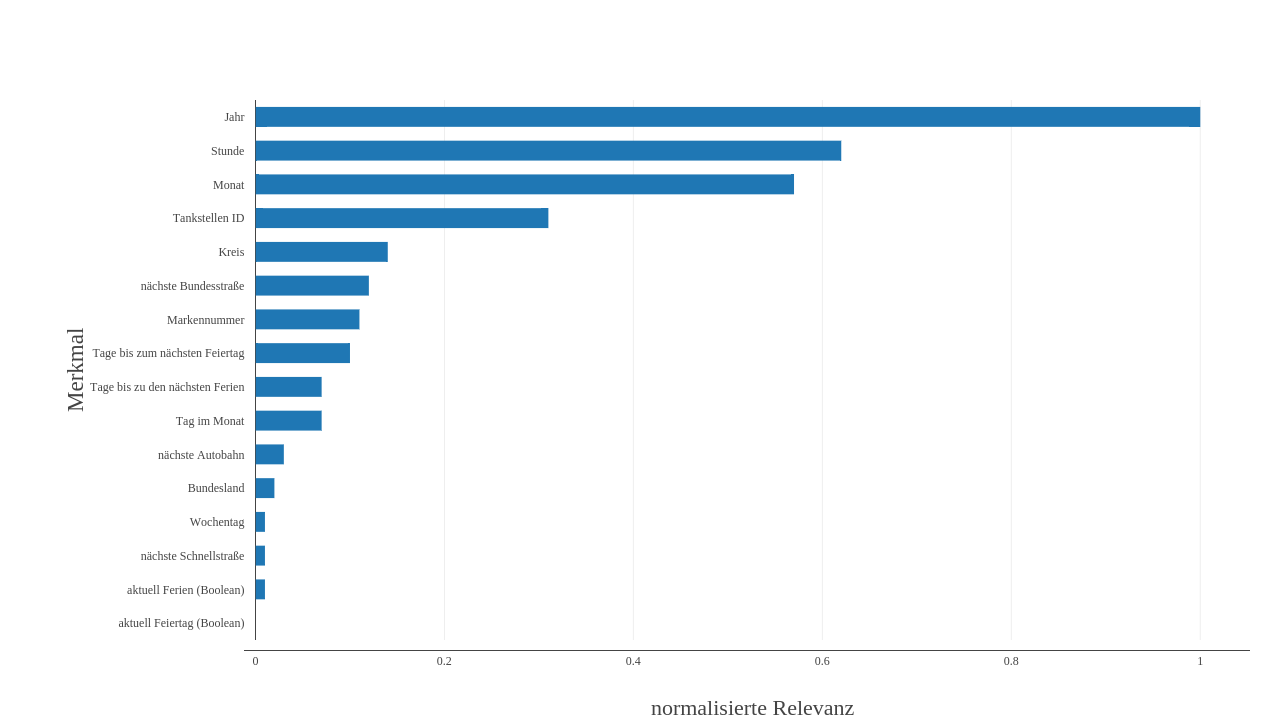
\includegraphics[width=\linewidth]{features720p.png}
\caption{Relative Relevanz der einzelnen Merkmale für die Vorhersage von Benzinpreisen.}
\label{fig:fi}
\end{figure}

\begin{figure}
\centering
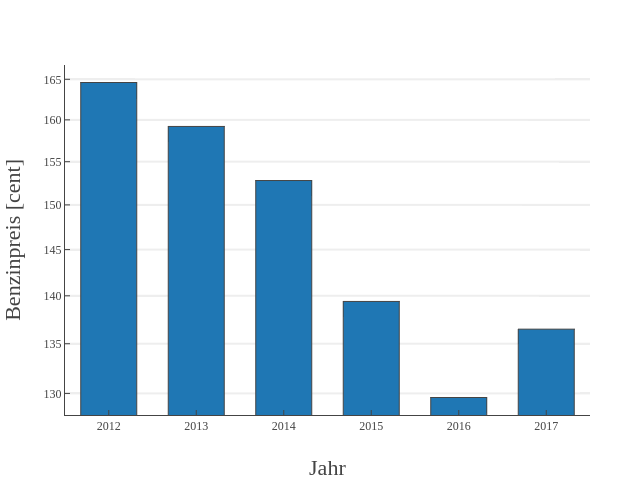
\includegraphics[width=0.7\linewidth]{Benzinpreisentwicklung_2012-2017.png}
\caption{Entwicklung der Jahresdurchschnittspreise für einen Liter Super Benzin in den Jahren 2012 bis 2017. Die Daten stammen von statista.com  \cite{stat}.}
\label{fig:bpe}
\end{figure}


\subsection{Modellauswahl}
Als erster Ansatz wurden unterschiedliche \ac{ARMA}-Modelle untersucht. Diese lassen jedoch keine Verwendung exogener Variablen zu, welche, wie später gezeigt, eine hohe Relevanz für die Vorhersage von Benzinpreisen besitzen. Anschließend wurden unterschiedliche maschinelle Lernverfahren untersucht, darunter auch einfache Deep-Learning Ansätze. Die manuelle Untersuchung dieser Algorithmen beansprucht jedoch viel Zeit. Um nicht unter Zeitdruck zu geraten, wurde die Modellsuche mit Hilfe der Open-Source Software H2O automatisiert. H2O implementiert Algorithmen aus den Bereichen Statistik, Data Mining und Maschinellem Lernen. Die Software basiert auf dem Hadoop Distributed File System, sodass ein Performance-Gewinn gegenüber anderen Analysewerkzeugen erzielt wird. \\
\par 
H2O kann mehrere Modelle des gleichen Typs mit anderen Modellen vergleichen und so das beste Modell für die gegebene Problemstellung finden. Durch ein Grid-Search werden die Hyperparameter der Modelle optimiert. Somit ist es möglich, in relativ kurzer Zeit ein wettbewerbsfähiges Modell zu erstellen. Für die gegebene Problemstellung hat sich ein Gradient Boosting Machine (GBM) Modell als besonders potent herausgestellt. Die Eigenschaften dieses Modells werden nachfolgend kurz erläutert.

\subsubsection*{Gradient Boosting Machine}
Die Erklärung der Gradient Boosting Machines erfolgt nach Friedmann \cite{gbm}. Durch Gradient Boosting wird ein Ensemble aus mehreren einfachen Modellen gebildet, welche als Aggregat ein neues und stärkeres Modell bilden. Die beinhalteten Modelle werden dabei so gebildet, dass der Gesamtfehler aller Modelle, inklusive des neu erstellten Modells, minimiert wird. Dies geschieht über den Gradienten der Fehlerfunktion unter Berücksichtigung der Vorhersage. Der Algorithmus funktioniert dabei wie folgt:

\begin{enumerate}
\item Ein Modell, üblicherweise ein Entscheidungsbaum, wird auf die Daten angepasst: 
\begin{equation*}
F_1(x) = y
\end{equation*}
\item Ein zweites Modell wird auf die Restwerte des ersten Modells angepasst:
\begin{equation*}
h_1(x) = y - F_1(x)
\end{equation*}
\item Aus diesen Modellen wird additiv ein neues Modell gebildet:
\begin{equation*}
F_2(x) = F_1(x) + h_1(x)
\end{equation*}
\end{enumerate}

Die grundlegende Idee dieses Boosting-Verfahrens ist es also, immer neue Modelle hinzuzufügen, die den Fehler des vorherigen Modells korrigieren. Das Modell wird über die Minimierung einer definierten Fehlerfunktion $L(y, F(x))$ trainiert. Diese Optimierung geschieht über ein Gradientenverfahren. Es ergeben sich folgende Aktualisierungsregeln:

\begin{equation*}
F_m(x) = F_{m-1}(x) - \gamma_m \sum_{i=1}^{n} \nabla_{F_m(x)} L(y_i, F_{m-1}(x_i))
\end{equation*}

Wobei $\gamma_m$ die Lernrate des aktuell betrachteten Modells repräsentiert. Diese Lernrate wird adaptiv nach folgender Vorschrift angepasst:

\begin{equation*}
\gamma_m = \argmin_\gamma \sum_{i=1}^{n} L\bigl(y_i, F_{m-1}(x) - \gamma \nabla_{F_m(x)} L(y_i, F_{m-1}(x_i))\bigr)
\end{equation*}

\subsubsection*{Ergebnisse der Grid Search}
Die Hyperparameter der implementierten GBM wurden durch eine Grid Search optimiert. \autoref{tab:params} gibt eine Übersicht über die wichtigsten Hyperparameter-Werte des Modells.

\begin{table}[h]
	\centering
	\begin{tabular}{l r}
		\textbf{Parameter} & \textbf{Wert} \\ 
		\hline \hline
		Anzahl an Entscheidungsbäumen & 50 \\ 
		Anzahl interner Bäume & 50  \\
		Minimale Tiefe & 5 \\
        Maximale Tiefe & 5\\
        Minimale Anzahl an Blättern & 32 \\
        Maximale Anzahl an Blättern & 32 \\
        K-fold cross validation & K=5 \\
        Lernrate & 0.1 \\
		\hline 
	\end{tabular}
	\caption{Die Hyperparameter-Werte des GBM-Modells, welche durch die Grid-Search optimiert wurden.}
	\label{tab:params}	
\end{table} 

\subsection{Training}
Da die ursprünglich als Zeitreihenvorhersage gedachte Aufgabenstellung durch eine Regressionsaufgabe substituiert werden konnte, trainiert das implementierte Modell mit dem gesamten Datensatz. Dies ist insbesondere für Preisvorhersagen, welche weit außerhalb der vorhandenen Datenbasis liegen von Vorteil. Der größte Nachteil an dieser Methode ist die benötigte Rechenpower. Die Trainingsmenge umfasst beinahe 15 Gigabyte. Da H2O den Datensatz komplett in den Arbeitsspeicher lädt, wird für das Training eine dementsprechend starke Rechenmaschine benötigt. Um dieses Modell zu trainieren, wurde daher auf eine Deep Learning Workstation mit 64 Gigabyte Arbeitsspeicher zurückgegriffen.\\
\par

Das Training des Modells erfolgte in einer fünffachen Kreuzvalidierung und dauerte etwas mehr als drei Stunden. Im Mittel besitzt das Modell noch einen \ac{RMSE} von 42.5 zehntel Cent auf den Testdaten. Dieser Wert ist durchaus passabel, da das Modell Preise unabhängig von deren vorheriger Entwicklung vorhersagen kann. In anderen Worten bedeutet dies, dass wir einen konstanten Fehler auf unseren Vorhersagen haben, welcher sich nicht bei schrittweisen Vorhersagen aufaddiert. 

\section{CLI}

Zum automatisierten Vergleich der Ergebnisse der Anwendung mit den Ergebnissen vergleichbarer Anwendungen wurde ein \ac{CLI} implementiert. Dieses \ac{CLI} benötigt Python 3.6 und ist im Unterordner \texttt{CLI} enthalten. Der Aufruf für die Berechnung einer Tankstrategie ist wie folgt:

\begin{lstlisting}
python cli.py --input pfad_zu_csv --output pfad_zu_output \
--host "http://localhost:4567" --type route
\end{lstlisting}

Für den Abruf einer Preisvorhersage kann Folgendes verwendet werden:

\begin{lstlisting}
python cli.py --input pfad_zu_csv --output pfad_zu_output \
--host "http://localhost:4567" --type pred
\end{lstlisting}

\chapter{Besonderheiten / Vorteile bei bestimmten Routen / Preisvorhersagen}

Dieses Kapitel geht auf Besonderheiten der Anwendung ein und schlägt Routen und Preisvorhersagen vor, die diese Besonderheiten hervorheben. Sämtliche vorgeschlagenen Routen und Preisvorhersagen sind im Ordner \path{routingService/src/test/resources/com/github/robinbaumann/informaticup2018} als \ac{CSV} Dateien enthalten. Die folgenden Abschnitte beschreiben jeweils in Tabellenform solche Daten.

Sämtliche hier beschriebenen Datensätze werden in den Integration Tests verwendet, um die Korrektheit des Verhaltens sicherzustellen.
\section{Fehlerfälle}
\subsection{Nicht existierende Tankstellen}

\begin{table}[H]
	\centering
	\begin{tabular}{l l}
    	\hline
		\textbf{Typ} & Tankstrategie \\ 
		\textbf{Dateiname} & bertha\_bogus\_station.csv \\
        \textbf{Besonderheit} & enthält eine Tankstellen Id, die es nicht gibt \\
        \textbf{Verhalten} & Anwendung antwortet mit entsprechender ProblemResponse, kein Absturz \\
		\hline 
	\end{tabular}
\end{table} 

\subsection{Leere Tankstrategie}

\begin{table}[H]
	\centering
	\begin{tabular}{l l}
    	\hline
		\textbf{Typ} & Tankstrategie \\ 
		\textbf{Dateiname} & bertha\_empty.csv \\
        \textbf{Besonderheit} & enthält nur die Kapazität \\
        \textbf{Verhalten} & Anwendung antwortet mit entsprechender ProblemResponse, kein Absturz \\
		\hline 
	\end{tabular}
\end{table} 

\subsection{Negative Tankkapazität}

\begin{table}[H]
	\centering
	\begin{tabular}{l l}
    	\hline
		\textbf{Typ} & Tankstrategie \\ 
		\textbf{Dateiname} & bertha\_negative\_capacity.csv \\
        \textbf{Besonderheit} & die Tankkapzität hat einen negativen Wert \\
        \textbf{Verhalten} & Anwendung antwortet mit entsprechender ProblemResponse, kein Absturz \\
		\hline 
	\end{tabular}
\end{table} 

\subsection{Tankstops sind nicht in zeitlicher Reihenfolge}

\begin{table}[H]
	\centering
	\begin{tabular}{l l}
    	\hline
		\textbf{Typ} & Tankstrategie \\ 
		\textbf{Dateiname} & bertha\_out\_of\_order.csv \\
        \textbf{Besonderheit} & zwei Tankstops wurden vertauscht, die Reihenfolge in der CSV \\
        & entspricht nicht der zeitlichen Reihenfolge \\
        \textbf{Verhalten} & Anwendung antwortet mit entsprechender ProblemResponse, kein Absturz \\
		\hline 
	\end{tabular}
\end{table} 

\subsection{Routen mit Tankstellen ohne Preisinformationen}

\begin{table}[H]
	\centering
	\begin{tabular}{l l}
    	\hline
		\textbf{Typ} & Tankstrategie \\ 
		\textbf{Dateiname} & bertha\_stations\_without\_prices.csv \\
        \textbf{Besonderheit} & Es werden Tankstellen angefragt für die in den Originaldaten \\ 
        & keine Preise hinterlegt waren \\
        \textbf{Verhalten} & Anwendung antwortet mit entsprechender ProblemResponse, kein Absturz \\
		\hline 
	\end{tabular}
\end{table} 

\subsection{Daten nach angefragtem Zeitpunkt verfügbar}

\begin{table}[H]
	\centering
	\begin{tabular}{l l}
    	\hline
		\textbf{Typ} & Preisvorhersage \\ 
		\textbf{Dateiname} & price-prediction-historic.csv \\
        \textbf{Besonderheit} & Es wird ein Preis angefragt und es können Daten bis nach dem angefragten Zeitpunkt \\
        & verwendet werden \\
        \textbf{Verhalten} & Anwendung antwortet mit dem tatsächlichen Preis zu dem Zeitpunkt \\
		\hline 
	\end{tabular}
\end{table} 


\subsection{Daten bis kurz vor angefragtem Zeitpunkt verfügbar}

\begin{table}[H]
	\centering
	\begin{tabular}{l l}
    	\hline
		\textbf{Typ} & Preisvorhersage \\ 
		\textbf{Dateiname} & price-prediction-very-close.csv \\
        \textbf{Besonderheit} & Es wird ein Preis angefragt und es können Daten bis kurz vor (1h) dem \\
        & angefragten Zeitpunkt verwendet werden \\
        \textbf{Verhalten} & Anwendung antwortet letztem tatsächlichen Preis zu dem Zeitpunkt \\
		\hline 
	\end{tabular}
\end{table} 

\subsection{Routen Stops nicht erreichbar mit vollem Tank}

\begin{table}[H]
	\centering
	\begin{tabular}{l l}
    	\hline
		\textbf{Typ} & Tankstrategie \\ 
		\textbf{Dateiname} & not-reachable.csv \\
        \textbf{Besonderheit} & An einer gewissen Position in der Route, ist der nächste Stopp selbst mit vollem Tank nicht erreichbar. \\
        \textbf{Verhalten} & Anwendung antwortet mit entsprechender ProblemResponse, kein Absturz \\
		\hline 
	\end{tabular}
\end{table} 


\section{Evaluation}

Zusätzlich zu den oben genannten Routen wurden noch vier weitere erstellt zur Evaluierung der hier implementierten Tankstrategie gegen die oben definierte naive Tankstrategie. Es werden nun vier Routen verglichen anhand der tatsächlichen Kosten, die nach den zwei Tankstrategien jeweils anfallen würden. Die Euro-Beträge sind auf die zweite Dezimalstelle und die Prozentwerte auf eine ganze Zahl gerundet.

\begin{table}[H]
	\centering
	\begin{tabular}{l l}
    	\hline
		\textbf{Typ} & Tankstrategie \\ 
		\textbf{Dateiname} & test1.csv \\
        \textbf{Naive Strategie} & 50.96€ \\
        \textbf{Optimale Strategie} & 25.70€ \\
  		\textbf{Günstiger} & 25.26€ \\
        \textbf{\% günstiger} & 50\% \\
		\hline 
	\end{tabular}
\end{table} 

\begin{table}[H]
	\centering
	\begin{tabular}{l l}
    	\hline
		\textbf{Typ} & Tankstrategie \\ 
		\textbf{Dateiname} & test2.csv \\
        \textbf{Naive Strategie} & 138.08€ \\
        \textbf{Optimale Strategie} & 56.02€ \\
  		\textbf{Günstiger} & 82.06€ \\
        \textbf{\% günstiger} & 40\% \\
		\hline 
	\end{tabular}
\end{table} 

\begin{table}[H]
	\centering
	\begin{tabular}{l l}
    	\hline
		\textbf{Typ} & Tankstrategie \\ 
		\textbf{Dateiname} & test3.csv \\
        \textbf{Naive Strategie} & 118.01€ \\
        \textbf{Optimale Strategie} & 68.17€ \\
  		\textbf{Günstiger} & 49.84€ \\
        \textbf{\% günstiger} & 57\% \\
		\hline 
	\end{tabular}
\end{table} 

\begin{table}[H]
	\centering
	\begin{tabular}{l l}
    	\hline
		\textbf{Typ} & Tankstrategie \\ 
		\textbf{Dateiname} & test4.csv \\
        \textbf{Naive Strategie} & 46.36€ \\
        \textbf{Optimale Strategie} & 28.08€ \\
  		\textbf{Differenz} & 18.28€ \\
        \textbf{\% günstiger} & 60\% \\
		\hline 
	\end{tabular}
\end{table} 

Im Schnitt ist bei unseren vier Testversuchen die optimale Tankstrategie 51.75\% günstiger als die naive.

\chapter{Ausblick}
Die vorgestellte Lösung hat seinen größten praktischen Nutzen sicherlich im Fernverkehr, insbesondere im Güterfernverkehr. Bei letzterem werden Lastkraftfahrzeuge eingesetzt, deren Tankkapazität mehrere hundert Liter umfasst. Durch die Benzinpreis-optimierte Routenplanung können hier erhebliche Kosten gespart werden. Ähnliches gilt für den Personenfernverkehr mit Bussen. Durch die eingesparten Spritkosten können Fahrkarten günstiger verkauft werden, was wiederum eventuell neue Kundschaft anlockt und somit in einer verstärkten Nutzung von Reisebussen resultiert. Dies hätte zusätzlich einen positiven ökologischen Nebeneffekt im Hinblick auf den Klimawandel. \\
\par
Die Planung des Bundesverkehrsministeriums zur Installation von 5000 Ladestationen für Elektroautos \cite{ladestations-planung} wirft die Überlegung in den Raum, ob Intellitank auch hierauf anwendbar ist. Mit dieser Investition soll auch ein einheitliches Bezahlsystem eingeführt werden. Laut einer Untersuchung der ISPEX AG \cite{oel-strom} folgt der Strompreis in seiner Entwicklung dem Ölpreis. Dies passt sehr gut in das Konzept von Intellitank. Probleme bereiten jedoch kostenlose Ladestationen für Supermarktkunden und die insgesamt noch limitierte Reichweite von Elektroautomobilen. Da der Besitzer sein Fahrzeug zu Hause aufladen kann, benötigt er für den Alltagsverkehr nicht zwingend ein Planungssystem für optimale Tankstrategien. Erst die flächendeckende Infrastruktur für Ladestationen macht Intellitank interessant für Besitzer von Elektrofahrzeugen, da sie somit auch über weite Strecken mit ihrem Fahrzeug reisen können. \\
\par 
Ein weiteres spannendes Einsatzgebiet für Intellitank bietet das Forschungsgebiet des Autonomous Driving. Ein selbstfahrendes Auto kann dann die Route Benzinpreis-optimal berechnen, so dass der Mitfahrer nur noch einsteigen muss und direkt losfahren kann. 

%-------------------------------------------------------------------------------
% APPENDIX
%-------------------------------------------------------------------------------
\newpage
\appendix

\chapter{Anleitungen}
\section*{Installationsanleitung}
\addcontentsline{toc}{section}{Installationsanleitung}
\label{label:installation}
Für die Installation wird von einem Linux System ausgegangen. Die Schritte sind für andere Betriebssysteme entsprechend anzupassen.

Zur Installation wird eine .zip-Datei namens 'RoutingService.zip' benötigt. Diese beinhaltet das Backend- und das Frontend-Setup, sowie eine fertig kompilierte Jar Datei.

Zusätzlich zu der .ZIP-Datei liegt anbei ein .sql-Dump.gz, welcher auf eine PostgreSql-Datenbank importiert werden muss. Die Anwendung wurde mit Postgresql 9.6.5 und PostGIS 2.3.3 getestet. Um die Datenbank aufzuspielen sind folgende Schritte notwendig.

\begin{lstlisting}
gunzip infocup.sql-dump.gz
psql infocup < infocup.sql-dump
\end{lstlisting}

Die Datenmenge ist recht groß. Deshalb sollte die Standardkonfiguration von Postgresql entsprechend angepasst werden.

Um die Jar Datei zu bauen wird das JDK8 und Maven benötigt. Während des Builds lädt Maven sowohl NodeJs als auch den Paket-Manager yarn herunter.

Um das Projekt zu generieren wird in den Ordner 'RoutingService' gewechselt und folgender Befehl ausgeführt:
\begin{lstlisting}
mvn clean install
\end{lstlisting}
Im Ordner {\em target} liegt nach erfolgreichem Build-Prozess die jar-Datei {\em RoutingService-1.0-SNAPSHOT.jar} vor.

\section*{Bedienungsanleitung}
\addcontentsline{toc}{section}{Bedienungsanleitung}

Um mit der Anwendung zu arbeiten, ohne selbst eine Datenbank aufzuspielen, kann die Demo Instanz genutzt werden. Diese ist unter \url{https://infocup.noshak.de} erreichbar. Der Benutzer \texttt{infocup} und das Passwort \texttt{predictp} werden für den Zugang benötigt.

Sofern die Installation aus vorherigem Abschnitt erfolgreich beendet wurde, kann man das Projekt mittels
\begin{lstlisting}
java -jar RoutingService-1.0-SNAPSHOT.jar \
  -D infocup.host="localhost:5432" \
  -D infocup.user="infocup"
\end{lstlisting}
starten.
Die übergebenen Properties \texttt{infocup.host} und \texttt{infocup.user} konfigurieren die Verbindung zur Datenbank und sind entsprechend anzupassen.

Wie in Abbildung \ref{fig:install1} zu sehen ist, gibt das Startup-Log die Adresse an, auf die der Server lauscht. In diesem Fall {\em 0.0.0.0:4567}, also abrufbar über {\em http://localhost:4567}.
\begin{figure}[H]
\centering
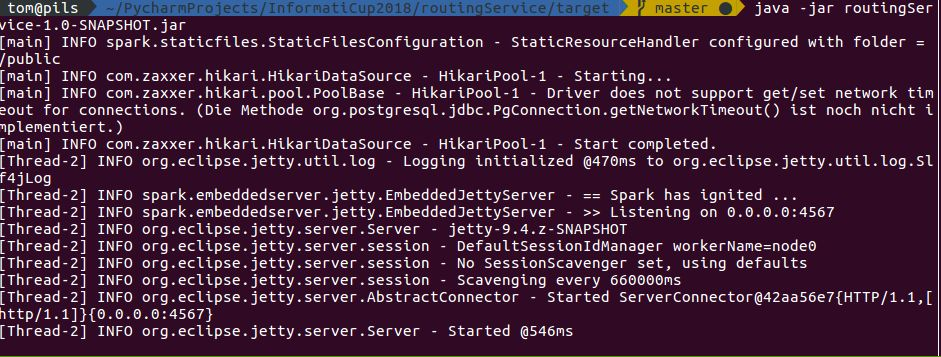
\includegraphics[width=1\linewidth]{install1.jpg}
\caption{Server-Log beim Starten des Projekts}
\label{fig:install1}
\end{figure}
Die Web-Anwendung bietet zwei wesentliche Funktionen.\\
Im unteren rechten Eck (siehe Abbildung \ref{fig:install2}) gibt es einen Button, der per Klick dem Benutzer die Möglichkeit eröffnet, entweder Preise vorherzusagen oder eine optimale Route berechnen zu lassen.
\begin{figure}[H]
\centering
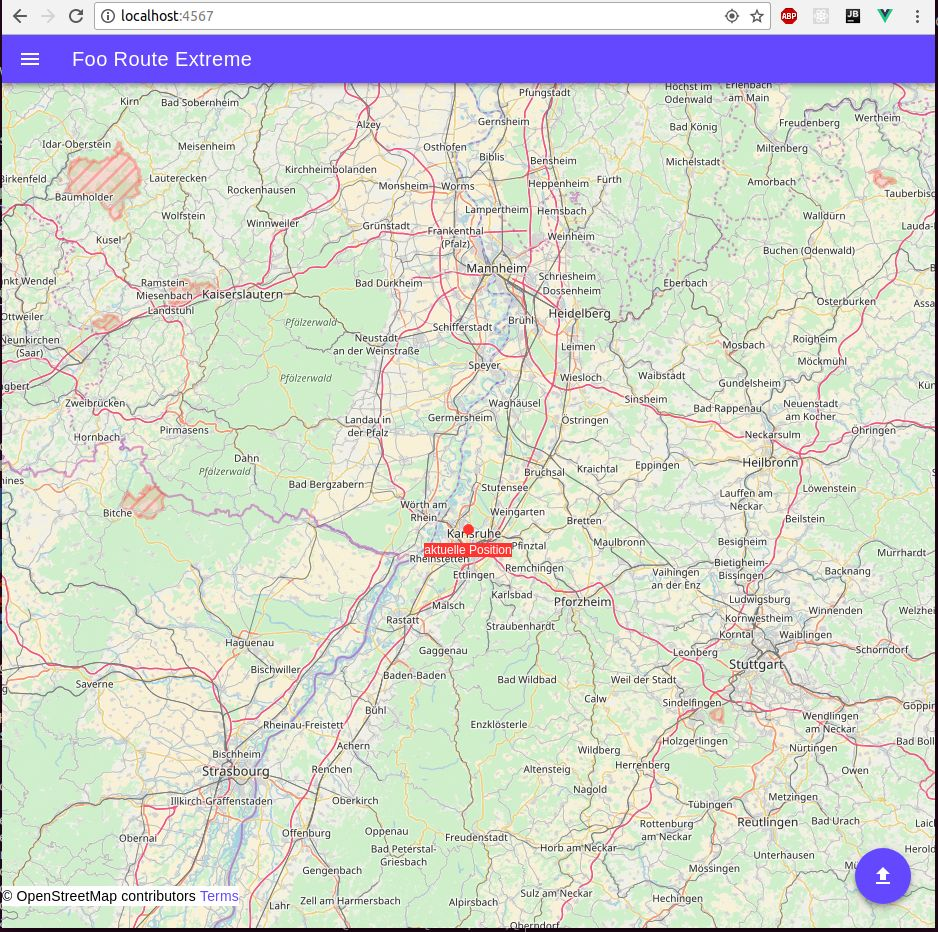
\includegraphics[width=0.6\linewidth]{install2.jpg}
\caption{grundlegende Oberfläche der Webanwendung}
\label{fig:install2}
\end{figure}
\clearpage

Die Buttons in Abbildung \ref{fig:install3} öffnen in beiden Fällen bei Klick einen File-Dialog zum Hochladen einer CSV-Datei.
Beim Klick auf den oberen Button besteht die Möglichkeit eine Tabelle, wie beispielsweise die Bertha-Benz-Memorial-Route, zu öffnen um eine optimale Tankstrategie zu berechnen. Beim Klick des unteren wird eine CSV-Datei erwartet, die Zeilen beinhaltet mit jeweils einer Tankstellen-ID und einem Datum, woraufhin eine Preisvorhersage berechnet wird.
\begin{figure}[H]
\centering
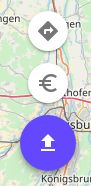
\includegraphics[width=50px]{install3.jpg}
\caption{die Benutzer-Interaktionsmöglichkeiten}
\label{fig:install3}
\end{figure}

\subsection{Routen-Berechnung}
Nach Eingabe der Bertha-Benz-Memorial-Route ist diese auf der Karte zu sehen (siehe Abbildung \ref{fig:install4}). Die Geo-Punkte der jeweiligen Tankstellen werden aus der Datenbank entnommen und auf die Karte projiziert. Ein blauer Punkt entspricht einer Tankstelle (Stopp), der grüne Punkt entspricht dem Startpunkt der Route, der beschriftete, rote Punkt der aktuellen Position und der zweite rote Punkt der letzten Station auf der Route.
\begin{figure}[H]
\centering
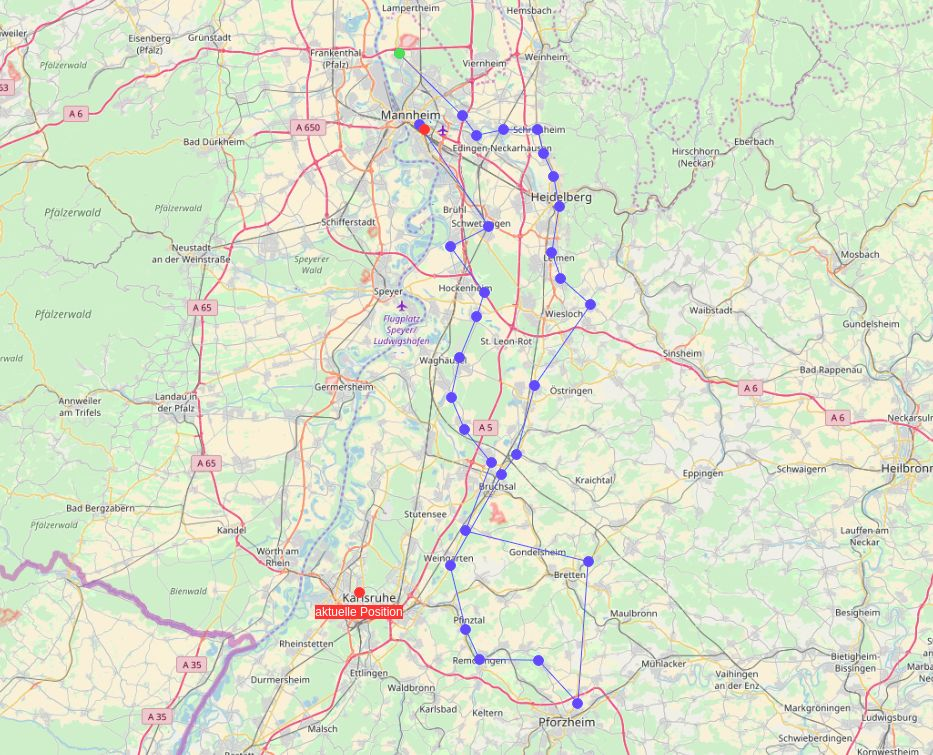
\includegraphics[width=0.6\linewidth]{install4.jpg}
\caption{Anzeige einer Tankroute}
\label{fig:install4}
\end{figure}
Neben der Karte kann ein Reiter eingeblendet werden, indem man den Navigations-Button oben links drückt (siehe Abbildung \ref{fig:install5}). Dieser dient dazu, die errechneten Tankfüllungen pro Routen-Stopp anzuzeigen.
\begin{figure}[H]
\centering
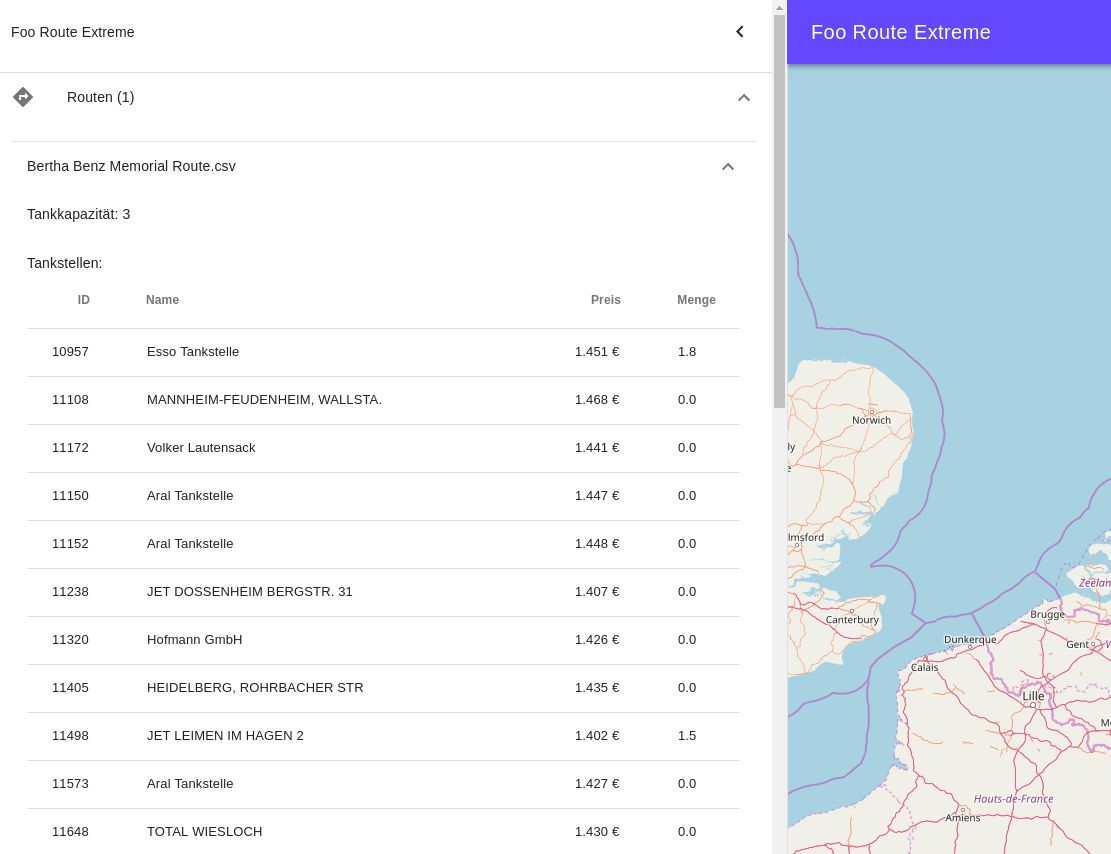
\includegraphics[width=0.8\linewidth]{install5.jpg}
\caption{die errechneten Tankfüllungen für die Route}
\label{fig:install5}
\end{figure}

\subsection{Preisvorhersage}

Wie auch bei der Routen-Berechnung werden bei der Funktion 'Preisvorhersage' alle Tankstellen in Form eines blauen Punktes auf der Karte illustriert (siehe Abbildung \ref{fig:install6}).
Der Unterschied ist jedoch, dass die jeweiligen Tankstellen nicht untereinander (wie bei einer Route) verbunden sind.
\begin{figure}[H]
\centering
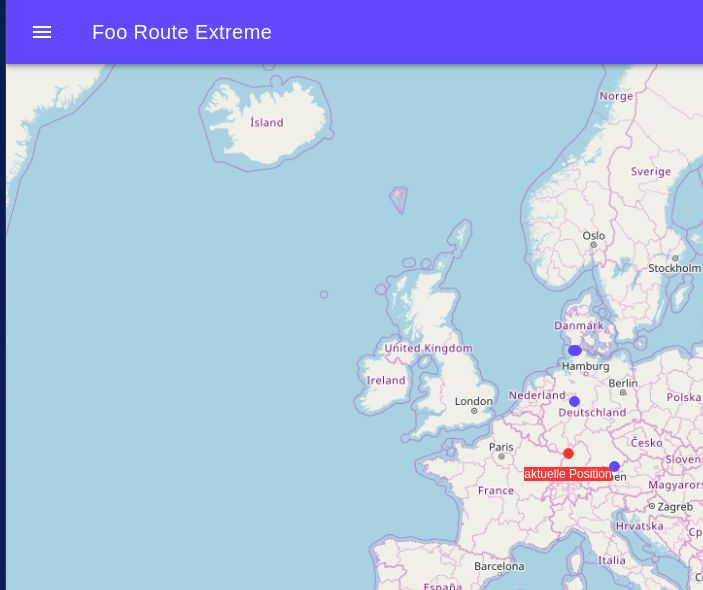
\includegraphics[width=0.6\linewidth]{install6.jpg}
\caption{die Tankstellen auf der Karte bei einer Preisvorhersage}
\label{fig:install6}
\end{figure}
Durch Klick auf die Top-Navigation, um den Reiter zu öffnen, werden die vorhergesagten Preise pro Tankstelle angezeigt (siehe Abb. \ref{fig:install7}).
\begin{figure}[H]
\centering
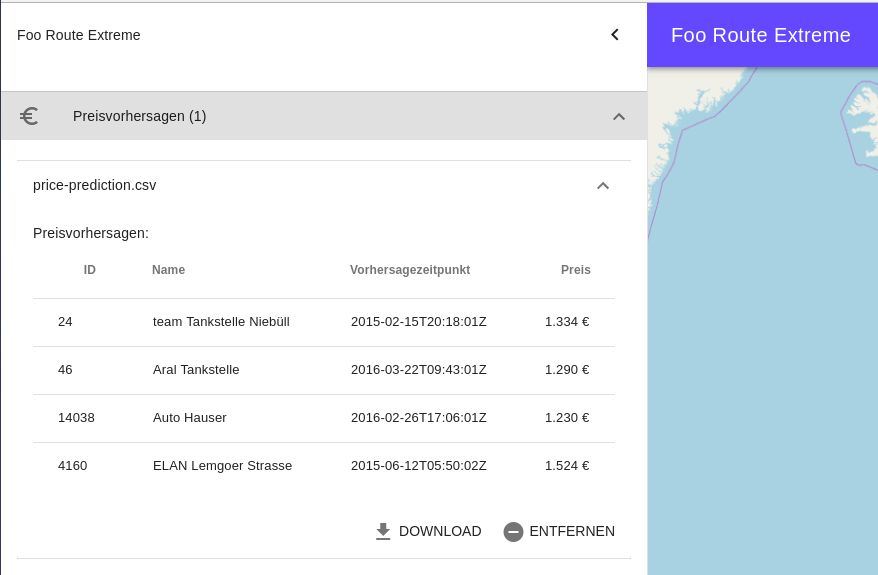
\includegraphics[width=0.8\linewidth]{install7.jpg}
\caption{die errechneten Preise zu den jeweiligen Daten}
\label{fig:install7}
\end{figure}

Zusätzlich bietet der Reiter die Möglichkeit die Routen zu löschen oder herunterzuladen.





%-------------------------------------------------------------------------------
% REFRENCES
%-------------------------------------------------------------------------------

\begin{thebibliography}{1}

\bibitem{fortbewegung} Brandt, Mathias {\em Auto ist in Deutschland immer noch die Nummer 1. statista.com \url{https://de.statista.com/infografik/9162/nutzung-von-verkehrsmitteln-in-deutschland/} (letzter Zugriff: 21.01.2018). 28.04.2017}.

\bibitem{holidays} {\em \texttt{holidays} Python Package, \url{https://pypi.python.org/pypi/holidays} (letzter Zugriff: 18.01.2018) }.

\bibitem{ferien} {\em Schulferien.org Website, \url{https://www.schulferien.org/} (letzter Zugriff: 18.01.2018) }.

\bibitem{osm} {\em OpenStreetMap.org Website \url{http://www.openstreetmap.org/} (letzter Zugriff: 18.01.2018)}.

\bibitem{faz} Siedenbeidel, Christian {\em Das Wunder des billigen Öls. Frankfurter allgemeine Zeitung. \url{http://www.faz.net/aktuell/finanzen/devisen-rohstoffe/wie-lange-autofahrer-noch-so-billig-tanken-koennen-13363092.html} (letzter Zugriff: 19.01.2018). 10.01.2015}.

\bibitem{stat} {\em statista.com Website \url{https://de.statista.com/statistik/daten/studie/776/umfrage/durchschnittspreis-fuer-superbenzin-seit-dem-jahr-1972/} (letzter Zugriff: 19.01.2018)}.

\bibitem{fixedgas} Khuller, Samir et. al {\em To Fill or not to Fill: The Gas Station Problem}.

\bibitem{nottingham} {\em Problem Details for HTTP APIs \url{https://tools.ietf.org/html/draft-nottingham-http-problem-06} (letzter Zugriff: 19.01.2018)}

\bibitem{gof} Erich Gamma, Richard Helm, Ralph Johnson, John Vlissides  {\em Design Patterns: Elements of Reusable Object-Oriented Software}  (10 November 1994)

\bibitem{haversine} {\em Haversine-Formel \url{https://rosettacode.org/wiki/Haversine_formula} (letzter Zugriff: 19.01.2018)}.

\bibitem{gbm} Friedmann, Jerome H. {\em Greedy Function Approximation: A Gradient Boosting Machine. The Annals of Statistics. 2001}

\bibitem{ladestations-planung} Schwarzer, Christoph M. {\em Das Ladeelend hat ein Ende. Zeit Online: \url{http://www.zeit.de/mobilitaet/2017-03/elektroauto-infrastruktur-bundesverkehrsministerium-foerdergeld-schnell-ladestationen} (letzter Zugriff: 20.01.2018). }

\bibitem{oel-strom} {\em Energiemarkt-Kommentar: Ölpreis dominiert alle Energiepreise. ISPEX AG Website \url{https://www.ispex.de/energiemarkt-kommentar-02-2016-oelpreis-dominiert-alle-energiepreise/} (letzter Zugriff: 20.01.2018).}

\end{thebibliography}

\end{document}

%-------------------------------------------------------------------------------
% SNIPPETS
%-------------------------------------------------------------------------------

%\begin{figure}[!ht]
%	\centering
%	\includegraphics[width=0.8\textwidth]{file_name}
%	\caption{}
%	\centering
%	\label{label:file_name}
%\end{figure}

%\begin{figure}[!ht]
%	\centering
%	\includegraphics[width=0.8\textwidth]{graph}
%	\caption{Blood pressure ranges and associated level of hypertension (American Heart Association, 2013).}
%	\centering
%	\label{label:graph}
%\end{figure}

%\begin{wrapfigure}{r}{0.30\textwidth}
%	\vspace{-40pt}
%	\begin{center}
%		\includegraphics[width=0.29\textwidth]{file_name}
%	\end{center}
%	\vspace{-20pt}
%	\caption{}
%	\label{label:file_name}
%\end{wrapfigure}

%\begin{wrapfigure}{r}{0.45\textwidth}
%	\begin{center}
%		\includegraphics[width=0.29\textwidth]{manometer}
%	\end{center}
%	\caption{Aneroid sphygmomanometer with stethoscope (Medicalexpo, 2012).}
%	\label{label:manometer}
%\end{wrapfigure}

%\begin{table}[!ht]\footnotesize
%	\centering
%	\begin{tabular}{cccccc}
%	\toprule
%	\multicolumn{2}{c} {Pearson's correlation test} & \multicolumn{4}{c} {Independent t-test} \\
%	\midrule	
%	\multicolumn{2}{c} {Gender} & \multicolumn{2}{c} {Activity level} & \multicolumn{2}{c} {Gender} \\
%	\midrule
%	Males & Females & 1st level & 6th level & Males & Females \\
%	\midrule
%	\multicolumn{2}{c} {BMI vs. SP} & \multicolumn{2}{c} {Systolic pressure} & \multicolumn{2}{c} {Systolic Pressure} \\
%	\multicolumn{2}{c} {BMI vs. DP} & \multicolumn{2}{c} {Diastolic pressure} & \multicolumn{2}{c} {Diastolic pressure} \\
%	\multicolumn{2}{c} {BMI vs. MAP} & \multicolumn{2}{c} {MAP} & \multicolumn{2}{c} {MAP} \\
%	\multicolumn{2}{c} {W:H ratio vs. SP} & \multicolumn{2}{c} {BMI} & \multicolumn{2}{c} {BMI} \\
%	\multicolumn{2}{c} {W:H ratio vs. DP} & \multicolumn{2}{c} {W:H ratio} & \multicolumn{2}{c} {W:H ratio} \\
%	\multicolumn{2}{c} {W:H ratio vs. MAP} & \multicolumn{2}{c} {\% Body fat} & \multicolumn{2}{c} {\% Body fat} \\
%	\multicolumn{2}{c} {} & \multicolumn{2}{c} {Height} & \multicolumn{2}{c} {Height} \\
%	\multicolumn{2}{c} {} & \multicolumn{2}{c} {Weight} & \multicolumn{2}{c} {Weight} \\
%	\multicolumn{2}{c} {} & \multicolumn{2}{c} {Heart rate} & \multicolumn{2}{c} {Heart rate} \\
%	\bottomrule
%	\end{tabular}
%	\caption{Parameters that were analysed and related statistical test performed for current study. BMI - body mass index; SP - systolic pressure; DP - diastolic pressure; MAP - mean arterial pressure; W:H ratio - waist to hip ratio.}
%	\label{label:tests}
%\end{table}